% \newcommand{\FigIdentifySender}{
% \begin{figure}[t]
%     \centering
%     \includegraphics[width=0.9\linewidth]{figures/linegraph.png}
%     \caption{\textbf{Messages needed to identify sender}\,---\,% 
%         We measured the number of epochs that were necessary for an attacker to
%         uniquely determine who was messaging a pre-selected victim, Bob, under
%         sealed sender assuming every message was ``immediately'' replied to with
%         a \textit{delivery receipt}. We found that the graph structure had no
%         influence on the effectiveness of the attack. We ran the attack 100
%         times for each user base size and found that with a user base of
%         1,000,000 on average Bob needed to receive 6.5 message from the same
%         user in order to deanonymize the conversation between the sender (Alice)
%         and Bob.
%         }
%     \label{fig:NumMessages}
% \end{figure}
% }

\newcommand{\IRTopDomainTable}{
    \begin{table}[t]
        \centering
        \begin{adjustbox}{width=\textwidth}
            \begin{tabular}{|c||ccc|}
                \hline\textbf{Domain} & \textbf{Requested Record Type} & \textbf{Number of Censoring v4 Resolvers} & \textbf{Number of Censoring v6 Resolvers}\\\hline
                secure.flickr.com & A & 276 & 209\\
                www.netflix.com & A & 275 & 206\\
                yumpu.com & A & 276 & 204\\
                www.urduvoa.com & A & 276 & 204\\
                www.snapchat.com & A & 274 & 206\\
                www.ning.com & A & 276 & 204\\
                www.lightsailvpn.com & A & 276 & 204\\
                signal.org & A & 275 & 205\\
                www.vonage.com & A & 276 & 203\\
                www.voanews.com & A & 276 & 203\\
                \hline
            \end{tabular}
        \end{adjustbox}
        \caption{\textbf{Iran table of most censored domains}\,---\,%
            We measured which domains were blocked in Iran, and whether they were
            blocked differently between resolvers at a v4 IP address, compared to
            those at a v6 IP address. As we can see here the most popularly blocked
            domains are blocked by resolvers on different IP address families but
            there is a difference. These domains were blocked by the most resolvers.
        }
        \label{tab:ir-top}
    \end{table}
}

\newcommand{\IRDifferenceDomainTable}{
    \begin{table}[ht]
        \centering
        \begin{adjustbox}{width=\textwidth}
            \begin{tabular}{|c||ccc|}
                \hline\textbf{Domain} & \textbf{Requested Record Type} & \textbf{Number of Censoring v4 Resolvers} & \textbf{Number of Censoring v6 Resolvers}\\\hline
                www.nbc.com & AAAA & 261 & 25\\
                download.cnet.com & AAAA & 259 & 23\\
                www.indiatimes.com & AAAA & 262 & 28\\
                spankbang.com & AAAA & 261 & 27\\
                psiphon.ca & AAAA & 261 & 27\\
                free.fr & AAAA & 261 & 27\\
                www.voanews.com & AAAA & 261 & 28\\
                www.netflix.com & AAAA & 262 & 29\\
                www.jesussaves.cc & AAAA & 261 & 28\\
                tmz.com & AAAA & 264 & 31\\
                \hline
            \end{tabular}
        \end{adjustbox}
        \caption{\textbf{Iran table of most difference in Address Family Censorship}\,---\,%
            We measured which domains were blocked in Iran, and whether they were
            blocked differently between resolvers at a v4 IP address, compared to
            those at a v6 IP address. As we can see here the most popularly blocked
            domains are blocked by resolvers on different IP address families but
            there is a difference. These domains had the largest difference in
            censoring behavior between resolver address family. 
        }
        \label{tab:ir-diff}
    \end{table}
}

\newcommand{\RUTopDomainTable}{
    \begin{table}[ht]
        \centering
        \begin{adjustbox}{width=\textwidth}
            \begin{tabular}{|c||ccc|}
                \hline\textbf{Domain} & \textbf{Requested Record Type} & \textbf{Number of Censoring v4 Resolvers} & \textbf{Number of Censoring v6 Resolvers}\\\hline
                eenadu.net & AAAA & 148 & 89\\
                www.spotify.com & AAAA & 93 & 98\\
                www.ned.org & A & 60 & 29\\
                www.europacasino.com & A & 47 & 37\\
                www.casinotropez.com & A & 45 & 37\\
                global.blackberry.com & A & 44 & 34\\
                www.sex.com & A & 40 & 37\\
                www.khilafah.com & A & 40 & 37\\
                ultrasurf.us & A & 41 & 36\\
                thepiratebay.org & A & 39 & 38\\
                \hline
            \end{tabular}
        \end{adjustbox}
        \caption{\textbf{Russia's top censored domains}\,---\,%
        }
        \label{tab:ru-top}
    \end{table}
}

\newcommand{\RUDifferenceDomainTable}{
    \begin{table}[ht]
        \centering
        \begin{adjustbox}{width=\textwidth}
            \begin{tabular}{|c||ccc|}
                \hline\textbf{Domain} & \textbf{Requested Record Type} & \textbf{Number of Censoring v4 Resolvers} & \textbf{Number of Censoring v6 Resolvers}\\\hline
                eenadu.net & AAAA & 148 & 89\\
                doh.dns.sb & A & 36 & 4\\
                www.ned.org & A & 60 & 29\\
                www.volcanomail.com & A & 30 & 0\\
                www.msf.org & A & 24 & 0\\
                mail.yahoo.com & A & 24 & 1\\
                www.cnn.com & AAAA & 0 & 21\\
                www.netflix.com & A & 27 & 10\\
                www.theglobalfund.org & A & 20 & 5\\
                www.ecdc.europa.eu & A & 15 & 0\\
                \hline
            \end{tabular}
        \end{adjustbox}
        \caption{\textbf{Russia's biggest difference domains}\,---\,%
        }
        \label{tab:ru-diff}
    \end{table}
}

\newcommand{\HKTopDomainTable}{
    \begin{table}[ht]
        \centering
        \begin{adjustbox}{width=\textwidth}
            \begin{tabular}{|c||ccc|}
                \hline\textbf{Domain} & \textbf{Requested Record Type} & \textbf{Number of Censoring v4 Resolvers} & \textbf{Number of Censoring v6 Resolvers}\\\hline
                eenadu.net & AAAA & 26 & 15\\
                www.ned.org & A & 14 & 3\\
                www.gov.uk & A & 12 & 2\\
                www.netflix.com & A & 11 & 2\\
                www.bittorrent.com & A & 10 & 2\\
                google.com.co & AAAA & 5 & 6\\
                www.nro.gov & A & 6 & 4\\
                www.terredeshommes.nl & A & 7 & 2\\
                mail.yahoo.com & A & 8 & 1\\
                google.ro & AAAA & 6 & 3\\
                \hline
            \end{tabular}
        \end{adjustbox}
        \caption{\textbf{Hong Kong's most censored domains}\,---\,%
        }
        \label{tab:hk-top}
    \end{table}
}

\newcommand{\HKDifferenceDomainTable}{
    \begin{table}[ht]
        \centering
        \begin{adjustbox}{width=\textwidth}
            \begin{tabular}{|c||ccc|}
                \hline\textbf{Domain} & \textbf{Requested Record Type} & \textbf{Number of Censoring v4 Resolvers} & \textbf{Number of Censoring v6 Resolvers}\\\hline
                www.ned.org & A & 14 & 3\\
                eenadu.net & AAAA & 26 & 15\\
                www.gov.uk & A & 12 & 2\\
                www.netflix.com & A & 11 & 2\\
                www.bittorrent.com & A & 10 & 2\\
                mail.yahoo.com & A & 8 & 1\\
                www.utorrent.com & A & 7 & 1\\
                www.ftchinese.com & A & 6 & 0\\
                www.familyequality.org & A & 7 & 1\\
                it.wikipedia.org & A & 6 & 0\\
                \hline
            \end{tabular}
        \end{adjustbox}
        \caption{\textbf{Hong Kong's biggest difference domains}\,---\,%
        }
        \label{tab:hk-diff}
    \end{table}
}

\newcommand{\CNTopDomainTable}{
    \begin{table}[ht]
        \centering
        \begin{adjustbox}{width=\textwidth}
            \begin{tabular}{|c||ccc|}
                \hline\textbf{Domain} & \textbf{Requested Record Type} & \textbf{Number of Censoring v4 Resolvers} & \textbf{Number of Censoring v6 Resolvers}\\\hline
                google.com.co & AAAA & 188 & 189\\
                google.co.in & AAAA & 189 & 188\\
                youtube.com & AAAA & 188 & 188\\
                www.ned.org & A & 189 & 187\\
                www.google.com & AAAA & 188 & 188\\
                www.blogger.com & AAAA & 188 & 188\\
                ultrasurf.us & AAAA & 188 & 188\\
                sites.google.com & AAAA & 188 & 188\\
                plus.google.com & AAAA & 188 & 188\\
                groups.google.com & AAAA & 188 & 188\\
                \hline
            \end{tabular}
        \end{adjustbox}
        \caption{\textbf{China's most censored domains}\,---\,%
        }
        \label{tab:cn-top}
    \end{table}
}

\newcommand{\CNDifferenceDomainTable}{
    \begin{table}[ht]
        \centering
        \begin{adjustbox}{width=\textwidth}
            \begin{tabular}{|c||ccc|}
                \hline\textbf{Domain} & \textbf{Requested Record Type} & \textbf{Number of Censoring v4 Resolvers} & \textbf{Number of Censoring v6 Resolvers}\\\hline
                google.com & A & 168 & 122\\
                google.com & AAAA & 180 & 145\\
                www.glaad.org & A & 30 & 6\\
                eenadu.net & AAAA & 116 & 96\\
                www.lanacion.com.ar & A & 20 & 1\\
                premierbet.co.ao & A & 25 & 7\\
                www.familyequality.org & A & 17 & 2\\
                www.bittorrent.com & A & 18 & 4\\
                qalam.withgoogle.com & A & 2 & 16\\
                global.blackberry.com & A & 16 & 2\\
                \hline
            \end{tabular}
        \end{adjustbox}
        \caption{\textbf{China's biggest difference domains}\,---\,%
        }
        \label{tab:cn-diff}
    \end{table}
}


% colors for the table below
%\definecolor{red0}{rgb}{1,0.9,0.9}
%\definecolor{red1}{rgb}{1,0.8,0.8}
%\definecolor{red2}{rgb}{1,0.7,0.7}
%\definecolor{red3}{rgb}{1,0.6,0.6}
%\definecolor{red4}{rgb}{1,0.5,0.5}
%\definecolor{red5}{rgb}{1,0.4,0.4}
%\definecolor{green0}{rgb}{0.9,1,0.9}
%\definecolor{green1}{rgb}{0.8,1,0.8}
%\definecolor{green2}{rgb}{0.7,1,0.7}
\definecolor{red00}{rgb}{1,0.9,0.9}
\definecolor{red0}{rgb}{1,0.8,0.8}
\definecolor{red1}{rgb}{1,0.7,0.7}
\definecolor{red2}{rgb}{1,0.6,0.6}
\definecolor{red3}{rgb}{1,0.5,0.5}
\definecolor{red4}{rgb}{1,0.4,0.4}
\definecolor{red5}{rgb}{1,0.3,0.3}
%\definecolor{green0}{rgb}{0.9,1,0.9}
\definecolor{green0}{rgb}{0.8,1,0.8}
\definecolor{green1}{rgb}{0.7,1,0.7}
\definecolor{green2}{rgb}{0.6,1,0.6}




\newcommand{\TabBaseRate}{
    \begin{table}[ht]
        \centering
        \small
        \scalebox{\tabularscale} {
        \begin{tabular}{lccccc}
            \toprule
                %\textbf{Country} & \textbf{Resolver pairs} & \textbf{v4/A} & \textbf{v4/AAAA} & \textbf{v6/A} & \textbf{v6/AAAA} \\
                \textbf{} & \textbf{Resolver} & \textbf{IPv4} & \textbf{IPv4} & \textbf{IPv6} & \textbf{IPv6} \\
                \textbf{Country} & \textbf{pairs} & \textbf{A} & \textbf{AAAA} & \textbf{A} & \textbf{AAAA} \\
                \midrule

United States (US)    &   1228  & 1.4\% & 0.9\% & 0.5\% & 0.9\% \\  % avg 0.9 stdev 2.6
Germany (DE)          &   753  & 1.0\% & 0.9\% & 0.8\% & 0.8\% \\  % avg 0.9 stdev 3.3
South Korea (KR)      &   632  & \cellcolor{red0} 2.3\% & 1.1\% & 1.2\% & 1.2\% \\  % avg 1.5 stdev 2.9
France (FR)           &   560  & 0.6\% & 0.5\% & 0.4\% & 0.6\% \\  % avg 0.5 stdev 1.8
Russia (RU)           &   312  & 5.5\% & 4.8\% & 4.5\% & 4.5\% \\  % avg 4.8 stdev 3.6
Iran (IR)             &   277  & \cellcolor{red1} 25.1\% & \cellcolor{red0} 24.5\% & \cellcolor{green0} 22.0\% & \cellcolor{green1} 21.4\% \\  % avg 23.3 stdev 3.4
Vietnam (VN)          &   252  & 1.5\% & 0.9\% & 1.4\% & 0.7\% \\  % avg 1.1 stdev 1.9
Taiwan (TW)           &   248  & 1.2\% & 1.0\% & 0.9\% & 0.9\% \\  % avg 1.0 stdev 4.0
India (IN)            &   226  & 1.3\% & 1.5\% & 1.0\% & 1.2\% \\  % avg 1.2 stdev 1.4
Canada (CA)           &   199  & \cellcolor{red0} 0.7\% & 0.4\% & 0.2\% & 0.3\% \\  % avg 0.4 stdev 1.2
United Kingdom (GB)   &   196  & 1.1\% & 0.9\% & 0.8\% & 1.0\% \\  % avg 1.0 stdev 3.3
China (CN)            &   194  & 29.3\% & \cellcolor{red0} 32.3\% & \cellcolor{green0} 28.4\% & \cellcolor{red0} 32.1\% \\  % avg 30.5 stdev 5.9
Thailand (TH)         &   186  & \cellcolor{red5}  8.2\% & \cellcolor{green0} 1.2\% & \cellcolor{green0} 1.1\% & \cellcolor{green0} 0.9\% \\  % avg 2.9 stdev 4.3
Brazil (BR)           &   160  & 2.7\% & 1.7\% & 2.0\% & 2.1\% \\  % avg 2.1 stdev 4.7
Japan (JP)            &   152  & 1.1\% & 1.2\% & 0.6\% & 1.0\% \\  % avg 1.0 stdev 3.4
Mexico (MX)           &   150  & \cellcolor{red0} 3.8\% & 2.0\% & 1.7\% & 1.9\% \\  % avg 2.4 stdev 5.0
Turkey (TR)           &   114  & 1.3\% & 1.0\% & 1.3\% & 1.0\% \\  % avg 1.1 stdev 3.2
Netherlands (NL)      &    97  & 1.2\% & 0.8\% & 0.7\% & 0.7\% \\  % avg 0.8 stdev 2.3
South Africa (ZA)     &    93  & 2.4\% & 1.6\% & 1.2\% & 1.4\% \\  % avg 1.6 stdev 4.2
Australia (AU)        &    72  & 1.6\% & 0.7\% & 0.9\% & 0.7\% \\  % avg 1.0 stdev 2.9
Hong Kong (HK)        &    67  & \cellcolor{red0} 7.0\% & 5.6\% & 4.9\% & 5.2\% \\  % avg 5.7 stdev 4.9
Chile (CL)            &    65  & \cellcolor{red1} 2.7\% & \cellcolor{green0} 0.7\% & 1.1\% & \cellcolor{green0} 0.8\% \\  % avg 1.3 stdev 1.8
Switzerland (CH)      &    60  & 0.3\% & 0.3\% & 0.3\% & 0.3\% \\  % avg 0.3 stdev 0.5
Indonesia (ID)        &    56  & \cellcolor{red0} 6.5\% & 3.0\% & 2.4\% & 2.3\% \\  % avg 3.5 stdev 6.3
Lithuania (LT)        &    52  & 0.9\% & 0.8\% & 0.5\% & 0.8\% \\  % avg 0.8 stdev 1.6
Singapore (SG)        &    50  & \cellcolor{red0} 1.8\% & 0.9\% & \cellcolor{green0} 0.6\% & 0.8\% \\  % avg 1.0 stdev 1.5
Malaysia (MY)         &    50  & \cellcolor{red1} 4.9\% & 2.0\% & \cellcolor{green0} 1.3\% & \cellcolor{green0} 1.4\% \\  % avg 2.4 stdev 3.5



                \hline
                %\textbf{Shown countries}            & \textbf{ 6501} & \textbf{3.8\%} & \textbf{3.2\%} & \textbf{2.8\%} & \textbf{3.0\%} \\
                \textbf{Global}            & \textbf{ 7441} & \textbf{3.6\%} & \textbf{3.0\%} & \textbf{2.6\%} & \textbf{2.7\%} \\
                \bottomrule
        \end{tabular}
        }
        \caption{\textbf{DNS censorship base rate}\,---\,%
            We discovered over 7,000 IPv4/IPv6 DNS resolver pairs around the world, and
            use them to measure censorship in their respective countries.
            We query each resolver pair (v4/v6 interfaces) with a list of over 700 domains
            from censorship lists that support both IPv4 and IPv6 addresses. For these domains,
            we request both \texttt{A} and \texttt{AAAA} records. We report on the average percent of censored
            responses for resolver inteface (v4 or v6) combined with record type (\texttt{A} or \texttt{AAAA}). Items significantly above (below) a country's average are colored red (green). We observe a general trend that IPv4 resolvers see more blocking than IPv6 resolvers.
            %and to a lesser extent, that IPv4 \texttt{A} records and IPv6 \texttt{AAAA} records are blocked more than IPv4 \texttt{AAAA} or IPv6 \texttt{A} records
            }
        \label{tab:base-rate}
    \end{table}
}


\newcommand{\TabBaseRateMedian}{
    \begin{table}[ht]
        \centering
        \small
        \scalebox{\tabularscale} {
        \begin{tabular}{lccccc}
            \toprule
                %\textbf{Country} & \textbf{Resolver pairs} & \textbf{v4/A} & \textbf{v4/AAAA} & \textbf{v6/A} & \textbf{v6/AAAA} \\
                \textbf{} & \textbf{Resolver} & \textbf{v4} & \textbf{v4} & \textbf{v6} & \textbf{v6} \\
                \textbf{Country} & \textbf{pairs} & \textbf{A} & \textbf{AAAA} & \textbf{A} & \textbf{AAAA} \\
                \midrule


                United States (US)    &   1228  & \cellcolor{green0} 0.1\% & 0.3\% & \cellcolor{green0} 0.1\% & 0.3\% \\  % avg 0.9 stdev 2.6 med 0.1
Germany (DE)          &   753  & 0.4\% & 0.4\% & 0.3\% & 0.4\% \\  % avg 0.9 stdev 3.3 med 0.4
South Korea (KR)      &   632  & 1.0\% & \cellcolor{green0} 0.6\% & \cellcolor{green0} 0.6\% & \cellcolor{green0} 0.6\% \\  % avg 1.5 stdev 2.9 med 0.6
France (FR)           &   560  & 0.1\% & 0.3\% & 0.1\% & 0.3\% \\  % avg 0.5 stdev 1.8 med 0.1
Russia (RU)           &   312  & 4.9\% & 4.9\% & 4.8\% & 4.9\% \\  % avg 4.8 stdev 3.6 med 4.9
Iran (IR)             &   277  & \cellcolor{red1} 25.4\% & \cellcolor{red0} 24.8\% & \cellcolor{green0} 21.8\% & \cellcolor{green0} 21.7\% \\  % avg 23.3 stdev 3.4 med 24.4
Vietnam (VN)          &   252  & 0.8\% & \cellcolor{green0} 0.4\% & \cellcolor{green0} 0.6\% & \cellcolor{green0} 0.4\% \\  % avg 1.1 stdev 1.9 med 0.6
Taiwan (TW)           &   248  & 0.3\% & 0.4\% & 0.3\% & 0.4\% \\  % avg 1.0 stdev 4.0 med 0.3
India (IN)            &   226  & 1.0\% & 1.0\% & \cellcolor{green0} 0.7\% & \cellcolor{green0} 0.8\% \\  % avg 1.2 stdev 1.4 med 0.8
Canada (CA)           &   199  & 0.3\% & 0.3\% & 0.1\% & 0.1\% \\  % avg 0.4 stdev 1.2 med 0.1
United Kingdom (GB)   &   196  & 0.3\% & 0.3\% & 0.1\% & 0.3\% \\  % avg 1.0 stdev 3.3 med 0.3
China (CN)            &   194  & \cellcolor{green0} 28.6\% & \cellcolor{red0} 32.1\% & \cellcolor{green0} 28.2\% & 31.9\% \\  % avg 30.5 stdev 5.9 med 31.4
Thailand (TH)         &   186  & \cellcolor{red5}  8.7\% & \cellcolor{green1} 0.6\% & \cellcolor{green1} 0.4\% & \cellcolor{green1} 0.4\% \\  % avg 2.9 stdev 4.3 med 0.6
Brazil (BR)           &   160  & \cellcolor{green0} 0.7\% & \cellcolor{green0} 0.6\% & \cellcolor{green0} 0.4\% & \cellcolor{green0} 0.6\% \\  % avg 2.1 stdev 4.7 med 0.6
Japan (JP)            &   152  & 0.1\% & 0.3\% & 0.1\% & 0.1\% \\  % avg 1.0 stdev 3.4 med 0.1
Mexico (MX)           &   150  & \cellcolor{green0} 0.4\% & \cellcolor{green0} 0.3\% & \cellcolor{green0} 0.1\% & \cellcolor{green0} 0.3\% \\  % avg 2.4 stdev 5.0 med 0.3
Turkey (TR)           &   114  & 0.7\% & 0.4\% & 0.4\% & 0.4\% \\  % avg 1.1 stdev 3.2 med 0.4
Netherlands (NL)      &    97  & \cellcolor{green0} 0.1\% & 0.3\% & \cellcolor{green0} 0.1\% & 0.3\% \\  % avg 0.8 stdev 2.3 med 0.3
South Africa (ZA)     &    93  & \cellcolor{green0} 0.4\% & 0.7\% & \cellcolor{green0} 0.3\% & \cellcolor{green0} 0.6\% \\  % avg 1.6 stdev 4.2 med 0.6
Australia (AU)        &    72  & 0.3\% & \cellcolor{green0} 0.1\% & \cellcolor{green0} 0.1\% & \cellcolor{green0} 0.1\% \\  % avg 1.0 stdev 2.9 med 0.1
Hong Kong (HK)        &    67  & 5.2\% & 4.8\% & 4.8\% & 4.8\% \\  % avg 5.7 stdev 4.9 med 4.8
Chile (CL)            &    65  & 1.3\% & \cellcolor{green0} 0.7\% & \cellcolor{green0} 0.7\% & \cellcolor{green0} 0.6\% \\  % avg 1.3 stdev 1.8 med 0.7
Switzerland (CH)      &    60  & \cellcolor{green0} 0.1\% & 0.3\% & \cellcolor{green0} 0.1\% & 0.3\% \\  % avg 0.3 stdev 0.5 med 0.1
Indonesia (ID)        &    56  & 4.9\% & \cellcolor{green0} 1.0\% & \cellcolor{green0} 1.0\% & \cellcolor{green0} 0.8\% \\  % avg 3.5 stdev 6.3 med 1.1
Lithuania (LT)        &    52  & 0.4\% & 0.6\% & 0.4\% & 0.4\% \\  % avg 0.8 stdev 1.6 med 0.4
Singapore (SG)        &    50  & 0.7\% & 0.7\% & \cellcolor{green0} 0.4\% & \cellcolor{green0} 0.6\% \\  % avg 1.0 stdev 1.5 med 0.6
Malaysia (MY)         &    50  & \cellcolor{red2} 5.2\% & \cellcolor{green0} 0.7\% & \cellcolor{green1} 0.4\% & \cellcolor{green1} 0.6\% \\  % avg 2.4 stdev 3.5 med 0.6

                \bottomrule
        \end{tabular}
        }
        \caption{\textbf{Base rate; medians}}
    \end{table}
}
 





\newcommand{\SomeCountryTable}{
    \begin{table}[ht]
        \centering
        \begin{tabular}{c|cc}
            \toprule
            \textbf{Country} & \textbf{Resolver pairs} & \textbf{Censored domains} \\
            \hline
                United States (US) & 1228 & 0\\
                Germany (DE) & 753 & 0\\
                South Korea (KR) & 632 & 0\\
                France (FR) & 560 & 0\\
                Russia (RU) & 312 & 30\\     % used to be 33??
                Iran (IR) & 277 & 169\\     % previously 172
                Vietnam (VN) & 252 & 0\\
                Taiwan (TW) & 248 & 0\\
                India (IN) & 226 & 0\\
                Canada (CA) & 199 & 0\\
                United Kingdom (GB) & 196 & 0\\
                China (CN) & 194 & 200\\
                Thailand (TH) & 186 & 0\\
                Brazil (BR) & 160 & 0\\
                Japan (JP) & 152 & 0\\
                Mexico (MX) & 150 & 0\\
                Turkey (TR) & 114 & 0\\     % used to be 3?
                Netherlands (NL) & 97 & 0\\
                South Africa (ZA) & 93 & 0\\
                Australia (AU) & 72 & 0\\
                Hong Kong (HK) & 67 & 30\\  % used to be 33
                Chile (CL) & 65 & 0\\
                Switzerland (CH) & 60 & 0\\
                Indonesia (ID) & 56 & 0\\
                Lithuania (LT) & 52 & 0\\
                Singapore (SG) & 50 & 0\\
                Malaysia (MY) & 50 & 0\\

                % UA & 35 & 1 \\        % dfas.mil
                % EG & 14 & 15 \\
                % KE & 8 & 2 \\
                % MO & 6 & 31 \\
                % AE & 6 & 6 \\
                % BY & 5 & 1 \\
                % TN & 2 & 1 \\
                % OM & 2 & 1 \\
                % MK & 2 & 47 \\
                % LA & 2 & 1 \\
                % IL & 2 & 30 \\
            \toprule
        \end{tabular}
        \caption{\textbf{DNS resolvers}\,---\,%
            We discovered over 7,000 IPv4/IPv6 DNS resolver pairs around the world, and
            use them to measure censorship in their respective countries.
            We queried each resolver with a list of over 700 domains from censorship
            lists that support both IPv4 and IPv6. We identify a domain as \texttt{censored}
            in a given country if over half of the country's resolvers blocked it.
            }
        \label{tab:country-resolvers}
    \end{table}
}

\newcommand{\FigIndiaCluster}{
    \begin{figure}[t]
     \centering
     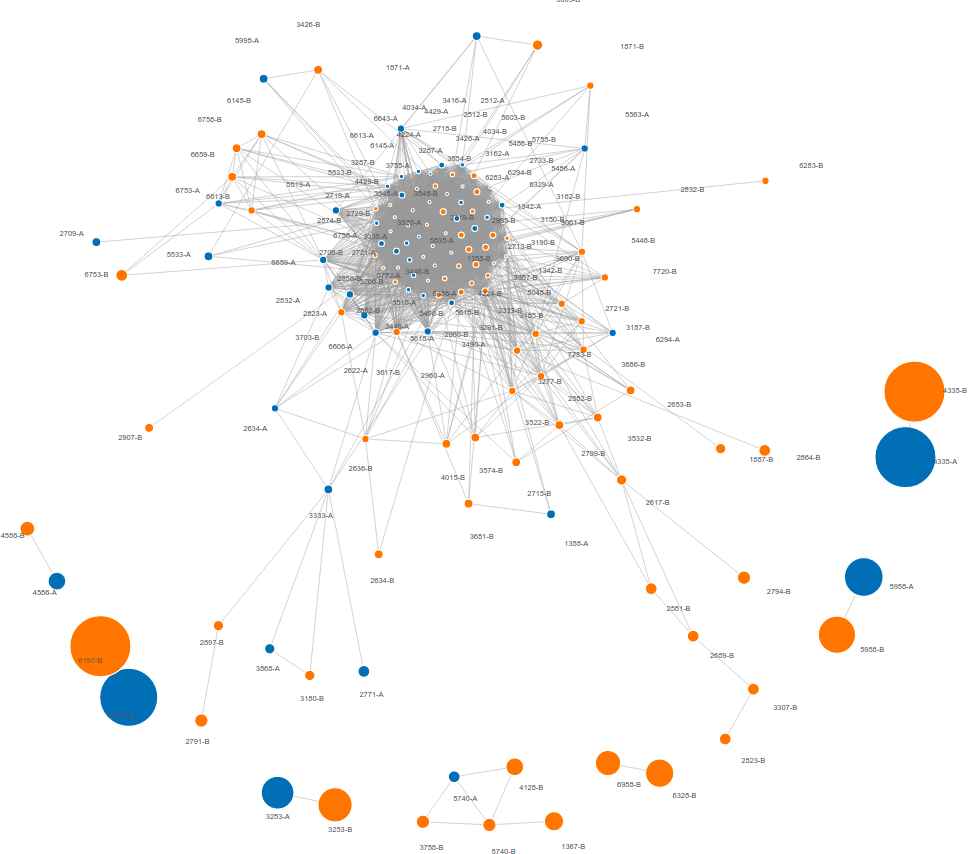
\includegraphics[width=0.9\linewidth]{figures/india.png}
     \caption{\textbf{India DNS censorship}\,---\,%
            We formed clusters of DNS resolvers using the levenshtein distance between
            the lists resolvers censor. Resolvers that block similar lists are connected,
            with node sizes proportional to the number of distinct domains blocked. We color
            IPv4 resolver interfaces blue, and IPv6 interfaces orange. This example illustrates
            the non-uniformity of India, with some ISPs censoring a large number of domains, and
            many others with small or non-existent block lists.}
    \label{fig:india}
    \end{figure}
}

\newcommand{\EveryCountryTable}{
    \begin{table}[ht]
        \centering
        {\tiny\renewcommand{\arraystretch}{.8}
        \resizebox{!}{.35\paperheight}{%
        \begin{tabular}{c|cc}
            \toprule
            \textbf{Country Code} & \textbf{Number of Resolver Pairs} & \textbf{Number of Censored Domains}\\
            \midrule
            US & 1228 & 0\\
            DE & 753 & 1\\
            KR & 632 & 2\\
            FR & 560 & 0\\
            RU & 312 & 33\\
            IR & 277 & 172\\
            VN & 252 & 2\\
            TW & 248 & 2\\
            IN & 226 & 2\\
            CA & 199 & 0\\
            GB & 196 & 0\\
            CN & 194 & 203\\
            TH & 186 & 2\\
            BR & 160 & 2\\
            JP & 152 & 0\\
            MX & 150 & 1\\
            TR & 114 & 3\\
            NL & 97 & 0\\
            ZA & 93 & 2\\
            AU & 72 & 0\\
            HK & 67 & 33\\
            CL & 65 & 2\\
            CH & 60 & 1\\
            ID & 56 & 2\\
            LT & 52 & 3\\
            SG & 50 & 3\\
            MY & 50 & 2\\
            ES & 49 & 0\\
            PL & 48 & 2\\
            AR & 47 & 2\\
            RO & 44 & 2\\
            CZ & 41 & 2\\
            IT & 38 & 1\\
            UA & 35 & 3\\
            SE & 34 & 0\\
            FI & 34 & 0\\
            BE & 31 & 1\\
            BG & 30 & 2\\
            BD & 29 & 3\\
            CO & 27 & 2\\
            SA & 24 & 2\\
            PK & 23 & 2\\
            HU & 22 & 1\\
            EC & 21 & 3\\
            GR & 20 & 0\\
            KZ & 19 & 0\\
            PH & 18 & 3\\
            NO & 16 & 0\\
            SK & 14 & 2\\
            EG & 14 & 17\\
            DK & 13 & 1\\
            PT & 11 & 0\\
            PE & 11 & 3\\
            NG & 9 & 2\\
            KE & 8 & 4\\
            AT & 8 & 1\\
            SI & 7 & 1\\
            RS & 7 & 0\\
            NZ & 7 & 1\\
            NP & 7 & 0\\
            MD & 7 & 0\\
            UY & 6 & 1\\
            MO & 6 & 32\\
            EE & 6 & 0\\
            CR & 6 & 3\\
            AE & 6 & 6\\
            VE & 5 & 2\\
            SD & 5 & 2\\
            PA & 5 & 0\\
            MN & 5 & 0\\
            LY & 5 & 1\\
            BY & 5 & 1\\
            AM & 5 & 1\\
            LV & 4 & 0\\
            LU & 4 & 0\\
            JO & 4 & 0\\
            IQ & 4 & 2\\
            GT & 4 & 0\\
            BZ & 4 & 1\\
            BO & 4 & 1\\
            BA & 4 & 1\\
            AL & 4 & 4\\
            LB & 3 & 1\\
            HR & 3 & 1\\
            HN & 3 & 1\\
            DO & 3 & 1\\
            AF & 3 & 0\\
            UG & 2 & 3\\
            TT & 2 & 0\\
            TN & 2 & 4\\
            TD & 2 & 2\\
            SV & 2 & 0\\
            OM & 2 & 2\\
            NI & 2 & 0\\
            MK & 2 & 49\\
            LA & 2 & 3\\
            IL & 2 & 31\\
            GU & 2 & 2\\
            GE & 2 & 2\\
            ET & 2 & 3\\
            CY & 2 & 3\\
            ZM & 1 & 5\\
            TZ & 1 & 4\\
            TG & 1 & 7\\
            SO & 1 & 1\\
            SC & 1 & 3\\
            PY & 1 & 8\\
            PF & 1 & 2\\
            MZ & 1 & 15\\
            MV & 1 & 11\\
            MM & 1 & 3\\
            MG & 1 & 7\\
            LK & 1 & 1\\
            LI & 1 & 1\\
            LC & 1 & 0\\
            KW & 1 & 1\\
            KG & 1 & 3\\
            HT & 1 & 0\\
            GI & 1 & 5\\
            GH & 1 & 2\\
            FJ & 1 & 2\\
            CM & 1 & 2\\
            AZ & 1 & 1\\
            AO & 1 & 4\\
            AI & 1 & 99\\
            PW & 0 & 3\\
            MA & 0 & 0\\
            KH & 0 & 4\\
            \bottomrule
        \end{tabular}}}
    \end{table}
}

\newcommand{\CompleteCountryTable}{
    \begin{table}[ht]
        \centering
        \begin{adjustbox}{width=\textwidth}
            \begin{tabular}{c|cc|cc|cc}
                \toprule
                \textbf{Country Code} & \textbf{Number of Resolver Pairs (January)} & \textbf{Number of Censored Domains (January)} & \textbf{Number of Resolver Pairs (December)} & \textbf{Number of Censored Domains (December)} & \textbf{Number of Resolver Pairs (November)} & \textbf{Number of Censored Domains (November)}\\
                \midrule
                US & 1228 & 0 & 1189 & 0 & 1201 & 0\\
                DE & 753 & 1 & 721 & 0 & 735 & 0\\
                KR & 632 & 2 & 504 & 2 & 595 & 2\\
                FR & 560 & 0 & 528 & 0 & 542 & 0\\
                RU & 312 & 33 & 296 & 32 & 316 & 33\\
                IR & 277 & 172 & 219 & 120 & 220 & 121\\
                VN & 252 & 2 & 179 & 2 & 214 & 2\\
                TW & 248 & 2 & 201 & 2 & 144 & 2\\
                IN & 226 & 2 & 181 & 2 & 185 & 2\\
                CA & 199 & 0 & 197 & 0 & 205 & 0\\
                GB & 196 & 0 & 196 & 0 & 190 & 0\\
                CN & 194 & 203 & 6 & 32 & 6 & 33\\
                TH & 186 & 2 & 144 & 3 & 202 & 2\\
                BR & 160 & 2 & 146 & 2 & 134 & 2\\
                JP & 152 & 0 & 138 & 0 & 142 & 0\\
                MX & 150 & 1 & 143 & 0 & 90 & 0\\
                TR & 114 & 3 & 90 & 2 & 102 & 2\\
                NL & 97 & 0 & 89 & 0 & 75 & 0\\
                ZA & 93 & 2 & 85 & 2 & 86 & 2\\
                AU & 72 & 0 & 65 & 0 & 71 & 0\\
                HK & 67 & 33 & 57 & 32 & 62 & 33\\
                CL & 65 & 2 & 46 & 2 & 63 & 2\\
                CH & 60 & 1 & 48 & 0 & 51 & 0\\
                ID & 56 & 2 & 31 & 2 & 53 & 2\\
                LT & 52 & 3 & 48 & 2 & 47 & 3\\
                SG & 50 & 3 & 29 & 2 & 39 & 3\\
                MY & 50 & 2 & 34 & 2 & 42 & 2\\
                ES & 49 & 0 & 46 & 0 & 54 & 0\\
                PL & 48 & 2 & 46 & 2 & 46 & 2\\
                AR & 47 & 2 & 47 & 2 & 55 & 2\\
                RO & 44 & 2 & 41 & 2 & 31 & 2\\
                CZ & 41 & 2 & 43 & 2 & 36 & 2\\
                IT & 38 & 1 & 29 & 0 & 31 & 0\\
                UA & 35 & 3 & 33 & 3 & 39 & 3\\
                SE & 34 & 0 & 34 & 0 & 35 & 0\\
                FI & 34 & 0 & 36 & 0 & 32 & 0\\
                BE & 31 & 1 & 32 & 0 & 26 & 0\\
                BG & 30 & 2 & 28 & 2 & 27 & 2\\
                BD & 29 & 3 & 7 & 3 & 21 & 2\\
                CO & 27 & 2 & 20 & 2 & 23 & 2\\
                SA & 24 & 2 & 15 & 2 & 11 & 2\\
                PK & 23 & 2 & 13 & 3 & 10 & 6\\
                HU & 22 & 1 & 16 & 0 & 15 & 1\\
                EC & 21 & 3 & 13 & 1 & 13 & 0\\
                GR & 20 & 0 & 13 & 0 & 15 & 0\\
                KZ & 19 & 0 & 14 & 1 & 21 & 0\\
                PH & 18 & 3 & 24 & 2 & 21 & 2\\
                NO & 16 & 0 & 16 & 0 & 13 & 0\\
                SK & 14 & 2 & 13 & 0 & 11 & 0\\
                EG & 14 & 17 & 13 & 16 & 2 & 27\\
                DK & 13 & 1 & 12 & 0 & 19 & 0\\
                PT & 11 & 0 & 15 & 0 & 11 & 0\\
                PE & 11 & 3 & 10 & 2 & 10 & 2\\
                NG & 9 & 2 & 7 & 3 & 6 & 2\\
                KE & 8 & 4 & 5 & 6 & 5 & 6\\
                AT & 8 & 1 & 11 & 0 & 8 & 1\\
                SI & 7 & 1 & 6 & 0 & 5 & 1\\
                RS & 7 & 0 & 6 & 0 & 4 & 0\\
                NZ & 7 & 1 & 5 & 0 & 6 & 0\\
                NP & 7 & 0 & 3 & 1 & 6 & 0\\
                MD & 7 & 0 & 5 & 0 & 1 & 1\\
                UY & 6 & 1 & 5 & 0 & 6 & 1\\
                MO & 6 & 32 & 7 & 31 & 4 & 31\\
                EE & 6 & 0 & 8 & 0 & 10 & 0\\
                CR & 6 & 3 & 6 & 2 & 4 & 0\\
                AE & 6 & 6 & 3 & 1 & 4 & 5\\
                VE & 5 & 2 & 4 & 2 & 5 & 2\\
                SD & 5 & 2 & 3 & 2 & 2 & 4\\
                PA & 5 & 0 & 3 & 0 & 4 & 0\\
                MN & 5 & 0 & 4 & 1 & 5 & 0\\
                LY & 5 & 1 & 4 & 3 & 5 & 2\\
                BY & 5 & 1 & 5 & 1 & 4 & 1\\
                AM & 5 & 1 & 2 & 5 & 2 & 1\\
                LV & 4 & 0 & 5 & 0 & 3 & 0\\
                LU & 4 & 0 & 3 & 0 & 3 & 0\\
                JO & 4 & 0 & 2 & 0 & 3 & 0\\
                IQ & 4 & 2 & 4 & 0 & 2 & 0\\
                GT & 4 & 0 & 5 & 0 & 6 & 0\\
                BZ & 4 & 1 & 3 & 1 & 2 & 1\\
                BO & 4 & 1 & 5 & 0 & 3 & 0\\
                BA & 4 & 1 & 3 & 1 & 3 & 0\\
                AL & 4 & 4 & 1 & 4 & 4 & 1\\
                LB & 3 & 1 & 2 & 0 & 2 & 0\\
                HR & 3 & 1 & 3 & 0 & 3 & 1\\
                HN & 3 & 1 & 3 & 0 & 1 & 0\\
                DO & 3 & 1 & 2 & 0 & 2 & 0\\
                AF & 3 & 0 & 2 & 3 & 3 & 4\\
                UG & 2 & 3 & 0 & -1 & 1 & 4\\
                TT & 2 & 0 & 2 & 1 & 2 & 0\\
                TN & 2 & 4 & 2 & 1 & 2 & 2\\
                TD & 2 & 2 & 2 & 2 & 2 & 2\\
                SV & 2 & 0 & 1 & 2 & 1 & 1\\
                OM & 2 & 2 & 1 & 2 & 1 & 0\\
                NI & 2 & 0 & 2 & 0 & 2 & 0\\
                MK & 2 & 49 & 1 & 2 & 2 & 50\\
                LA & 2 & 3 & 1 & 4 & 3 & 2\\
                IL & 2 & 31 & 4 & 0 & 4 & 0\\
                GU & 2 & 2 & 2 & 3 & 2 & 2\\
                GE & 2 & 2 & 2 & 3 & 3 & 1\\
                ET & 2 & 3 & 2 & 6 & 2 & 1\\
                CY & 2 & 3 & 2 & 2 & 3 & 3\\
                ZM & 1 & 5 & 0 & -1 & 0 & -1\\
                TZ & 1 & 4 & 1 & 5 & 1 & 7\\
                TG & 1 & 7 & 0 & -1 & 0 & 6\\
                SO & 1 & 1 & 1 & 3 & 1 & 2\\
                SC & 1 & 3 & 2 & 3 & 1 & 4\\
                PY & 1 & 8 & 2 & 7 & 2 & 6\\
                PF & 1 & 2 & 1 & 3 & 1 & 2\\
                MZ & 1 & 15 & 1 & 24 & 0 & -1\\
                MV & 1 & 11 & 0 & -1 & 0 & -1\\
                MM & 1 & 3 & 0 & -1 & 0 & -1\\
                MG & 1 & 7 & 1 & 5 & 2 & 6\\
                LK & 1 & 1 & 1 & 1 & 0 & -1\\
                LI & 1 & 1 & 1 & 1 & 1 & 2\\
                LC & 1 & 0 & 0 & -1 & 1 & 0\\
                KW & 1 & 1 & 1 & 1 & 1 & 1\\
                KG & 1 & 3 & 2 & 4 & 1 & 3\\
                HT & 1 & 0 & 0 & -1 & 0 & -1\\
                GI & 1 & 5 & 1 & 7 & 1 & 3\\
                GH & 1 & 2 & 1 & 2 & 2 & 2\\
                FJ & 1 & 2 & 0 & -1 & 0 & -1\\
                CM & 1 & 2 & 0 & -1 & 0 & -1\\
                AZ & 1 & 1 & 1 & 1 & 1 & 1\\
                AO & 1 & 4 & 1 & 2 & 1 & 3\\
                AI & 1 & 99 & 0 & -1 & 0 & -1\\
                PW & 0 & 3 & 1 & 1 & 1 & 1\\
                MA & 0 & 0 & 0 & 0 & 0 & -1\\
                KH & 0 & 4 & 3 & 2 & 0 & -1\\
                \bottomrule
            \end{tabular}
        \end{adjustbox}
    \end{table}
}

%%% Local Variables:
%%% mode: latex
%%% TeX-master: "main"
%%% End:
